% Options for packages loaded elsewhere
\PassOptionsToPackage{unicode}{hyperref}
\PassOptionsToPackage{hyphens}{url}
\PassOptionsToPackage{dvipsnames,svgnames,x11names}{xcolor}
%
\documentclass[
  letterpaper,
  DIV=11,
  numbers=noendperiod]{scrartcl}

\usepackage{amsmath,amssymb}
\usepackage{iftex}
\ifPDFTeX
  \usepackage[T1]{fontenc}
  \usepackage[utf8]{inputenc}
  \usepackage{textcomp} % provide euro and other symbols
\else % if luatex or xetex
  \usepackage{unicode-math}
  \defaultfontfeatures{Scale=MatchLowercase}
  \defaultfontfeatures[\rmfamily]{Ligatures=TeX,Scale=1}
\fi
\usepackage{lmodern}
\ifPDFTeX\else  
    % xetex/luatex font selection
\fi
% Use upquote if available, for straight quotes in verbatim environments
\IfFileExists{upquote.sty}{\usepackage{upquote}}{}
\IfFileExists{microtype.sty}{% use microtype if available
  \usepackage[]{microtype}
  \UseMicrotypeSet[protrusion]{basicmath} % disable protrusion for tt fonts
}{}
\makeatletter
\@ifundefined{KOMAClassName}{% if non-KOMA class
  \IfFileExists{parskip.sty}{%
    \usepackage{parskip}
  }{% else
    \setlength{\parindent}{0pt}
    \setlength{\parskip}{6pt plus 2pt minus 1pt}}
}{% if KOMA class
  \KOMAoptions{parskip=half}}
\makeatother
\usepackage{xcolor}
\setlength{\emergencystretch}{3em} % prevent overfull lines
\setcounter{secnumdepth}{5}
% Make \paragraph and \subparagraph free-standing
\makeatletter
\ifx\paragraph\undefined\else
  \let\oldparagraph\paragraph
  \renewcommand{\paragraph}{
    \@ifstar
      \xxxParagraphStar
      \xxxParagraphNoStar
  }
  \newcommand{\xxxParagraphStar}[1]{\oldparagraph*{#1}\mbox{}}
  \newcommand{\xxxParagraphNoStar}[1]{\oldparagraph{#1}\mbox{}}
\fi
\ifx\subparagraph\undefined\else
  \let\oldsubparagraph\subparagraph
  \renewcommand{\subparagraph}{
    \@ifstar
      \xxxSubParagraphStar
      \xxxSubParagraphNoStar
  }
  \newcommand{\xxxSubParagraphStar}[1]{\oldsubparagraph*{#1}\mbox{}}
  \newcommand{\xxxSubParagraphNoStar}[1]{\oldsubparagraph{#1}\mbox{}}
\fi
\makeatother


\providecommand{\tightlist}{%
  \setlength{\itemsep}{0pt}\setlength{\parskip}{0pt}}\usepackage{longtable,booktabs,array}
\usepackage{calc} % for calculating minipage widths
% Correct order of tables after \paragraph or \subparagraph
\usepackage{etoolbox}
\makeatletter
\patchcmd\longtable{\par}{\if@noskipsec\mbox{}\fi\par}{}{}
\makeatother
% Allow footnotes in longtable head/foot
\IfFileExists{footnotehyper.sty}{\usepackage{footnotehyper}}{\usepackage{footnote}}
\makesavenoteenv{longtable}
\usepackage{graphicx}
\makeatletter
\newsavebox\pandoc@box
\newcommand*\pandocbounded[1]{% scales image to fit in text height/width
  \sbox\pandoc@box{#1}%
  \Gscale@div\@tempa{\textheight}{\dimexpr\ht\pandoc@box+\dp\pandoc@box\relax}%
  \Gscale@div\@tempb{\linewidth}{\wd\pandoc@box}%
  \ifdim\@tempb\p@<\@tempa\p@\let\@tempa\@tempb\fi% select the smaller of both
  \ifdim\@tempa\p@<\p@\scalebox{\@tempa}{\usebox\pandoc@box}%
  \else\usebox{\pandoc@box}%
  \fi%
}
% Set default figure placement to htbp
\def\fps@figure{htbp}
\makeatother
% definitions for citeproc citations
\NewDocumentCommand\citeproctext{}{}
\NewDocumentCommand\citeproc{mm}{%
  \begingroup\def\citeproctext{#2}\cite{#1}\endgroup}
\makeatletter
 % allow citations to break across lines
 \let\@cite@ofmt\@firstofone
 % avoid brackets around text for \cite:
 \def\@biblabel#1{}
 \def\@cite#1#2{{#1\if@tempswa , #2\fi}}
\makeatother
\newlength{\cslhangindent}
\setlength{\cslhangindent}{1.5em}
\newlength{\csllabelwidth}
\setlength{\csllabelwidth}{3em}
\newenvironment{CSLReferences}[2] % #1 hanging-indent, #2 entry-spacing
 {\begin{list}{}{%
  \setlength{\itemindent}{0pt}
  \setlength{\leftmargin}{0pt}
  \setlength{\parsep}{0pt}
  % turn on hanging indent if param 1 is 1
  \ifodd #1
   \setlength{\leftmargin}{\cslhangindent}
   \setlength{\itemindent}{-1\cslhangindent}
  \fi
  % set entry spacing
  \setlength{\itemsep}{#2\baselineskip}}}
 {\end{list}}
\usepackage{calc}
\newcommand{\CSLBlock}[1]{\hfill\break\parbox[t]{\linewidth}{\strut\ignorespaces#1\strut}}
\newcommand{\CSLLeftMargin}[1]{\parbox[t]{\csllabelwidth}{\strut#1\strut}}
\newcommand{\CSLRightInline}[1]{\parbox[t]{\linewidth - \csllabelwidth}{\strut#1\strut}}
\newcommand{\CSLIndent}[1]{\hspace{\cslhangindent}#1}

\KOMAoption{captions}{tableheading}
\makeatletter
\@ifpackageloaded{caption}{}{\usepackage{caption}}
\AtBeginDocument{%
\ifdefined\contentsname
  \renewcommand*\contentsname{Table of contents}
\else
  \newcommand\contentsname{Table of contents}
\fi
\ifdefined\listfigurename
  \renewcommand*\listfigurename{List of Figures}
\else
  \newcommand\listfigurename{List of Figures}
\fi
\ifdefined\listtablename
  \renewcommand*\listtablename{List of Tables}
\else
  \newcommand\listtablename{List of Tables}
\fi
\ifdefined\figurename
  \renewcommand*\figurename{Figure}
\else
  \newcommand\figurename{Figure}
\fi
\ifdefined\tablename
  \renewcommand*\tablename{Table}
\else
  \newcommand\tablename{Table}
\fi
}
\@ifpackageloaded{float}{}{\usepackage{float}}
\floatstyle{ruled}
\@ifundefined{c@chapter}{\newfloat{codelisting}{h}{lop}}{\newfloat{codelisting}{h}{lop}[chapter]}
\floatname{codelisting}{Listing}
\newcommand*\listoflistings{\listof{codelisting}{List of Listings}}
\makeatother
\makeatletter
\makeatother
\makeatletter
\@ifpackageloaded{caption}{}{\usepackage{caption}}
\@ifpackageloaded{subcaption}{}{\usepackage{subcaption}}
\makeatother

\usepackage{bookmark}

\IfFileExists{xurl.sty}{\usepackage{xurl}}{} % add URL line breaks if available
\urlstyle{same} % disable monospaced font for URLs
\hypersetup{
  pdftitle={Dosage Inequity in Pharmaceutical Studies: A Power Analysis},
  pdfauthor={Susan Peck; Jan Blackburn; Joseph Burks},
  colorlinks=true,
  linkcolor={blue},
  filecolor={Maroon},
  citecolor={Blue},
  urlcolor={Blue},
  pdfcreator={LaTeX via pandoc}}


\title{Dosage Inequity in Pharmaceutical Studies: A Power
Analysis\thanks{Project repository available at:
https://github.com/susanpeck/Math261BExperimentalDesignProject}}
\usepackage{etoolbox}
\makeatletter
\providecommand{\subtitle}[1]{% add subtitle to \maketitle
  \apptocmd{\@title}{\par {\large #1 \par}}{}{}
}
\makeatother
\subtitle{Replication and Reanalysis}
\author{Susan Peck \and Jan Blackburn \and Joseph Burks}
\date{May 9, 2026}

\begin{document}
\maketitle
\begin{abstract}
Clinical trials are often powered to detect overall treatment effects,
but not treatment effect differences within demographic subgroups. This
paper reanalyzes the ACTG 320 HIV clinical trial to evaluate whether sex
and race/ethnicity subgroups had adequate statistical power to support
subgroup-specific conclusions. Using Cox proportional hazards models,
Kaplan--Meier curves, likelihood ratio tests, and Schoenfeld-based power
calculations, we replicate the original overall treatment finding and
then assess subgroup treatment effects. Indinavir-containing therapy
reduced the hazard of AIDS progression or death by approximately 48\% in
the full sample, but most subgroup analyses were underpowered because
statistical information in survival analysis depends primarily on
observed events rather than enrollment counts. The female subgroup and
overall sample exceeded 80\% power, while the male, Hispanic,
Asian/Pacific Islander, and Other subgroups had too few events to
support reliable inference. These results show that demographic
representation alone does not guarantee inferential capacity and that
future trials should use event-driven subgroup targets when
subgroup-specific inference is a design objective.
\end{abstract}


\section{Introduction}\label{introduction}

Clinical trials are used for evaluating treatment efficacy, but they are
typically designed and powered to detect treatment effects in the
overall enrolled population. This means that demographic subgroups such
as women and\\
minorities are often enrolled in numbers too small to support reliable
inference about whether a treatment works equally well, or works at all,
for those groups. When a trial lacks the power to detect subgroup
differences, the absence of a significant finding cannot be interpreted
as evidence that the treatment effect is the same across all subgroups.
Yet the treatment guidelines are often generalized to all demographic
groups. .

The ACTG 320 trial (Hammer et al. 1997) is a HIV clinical trial that
provides an instructive case study for examining these limitations. ACTG
320 randomized 1,156 patients with advanced HIV disease to either a
standard two-drug nucleoside regimen or a three-drug regimen adding the
protease inhibitor indinavir. The trial was powered for an overall
treatment comparison and successfully demonstrated that indinavir
containing therapy reduced the hazard of AIDS progression or death by
approximately 50\%. However, enrollment was highly imbalanced across
demographic groups, with female participants comprising over 80\% of the
sample and several subgroups represented by only a handful of
participants and even fewer observed events.

The paper is going to investigate if the demographic subgroups were
adequately powered to detect treatment effects, and was indinavir's
benefit consistent across subgroups. In addition, what enrollment would
be required in a future study to achieve adequate power for all
demographic subgroups? In studies like ACTG 320 survival analysis is
driven by the number of observed events, not enrollment counts alone. A
subgroup can be proportionally represented in a trial while still
contributing too few events to support stable hazard ratio estimation or
meaningful hypothesis testing.

This paper first replicates the original ACTG 320 survival analysis
using Cox proportional hazards models and Kaplan--Meier curves, then
extends it through a systematic investigation of sex and race/ethnicity
subgroup treatment effects and prospective power analyses. The key
finding is that while the overall treatment effect and the female
subgroup were adequately powered, the male, Asian/Pacific Islander,
Hispanic, and Other race subgroups were not. The paper will describe
relevant literature on demographic representation in clinical trials
(Section~\ref{sec-lit-review}). It will then outline the ACTG 320 study
design (Section~\ref{sec-study-design}) and present the statistical
analysis plan and power analysis framework (Section~\ref{sec-methods}).
The reanalysis results are presented in (Section~\ref{sec-results}), and
findings, limitations, and implications for future trial design are
discussed in (Section~\ref{sec-discussion}).

\section{Literature Review}\label{sec-lit-review}

The underrepresentation of women and racial and ethnic minorities in
clinical trials has been documented across decades of pharmaceutical
research. Three studies are briefly described here.

Poon et al. (2013) examined women's participation and the reporting of
sex-stratified analyses in 156 late-phase trials supporting FDA approval
from 2000 to 2009. Women made up 45\% of participants on average, with
the greatest imbalances in cardiovascular and infectious disease trials.
Even when women were enrolled in adequate numbers, sex-specific results
were rarely reported. Fewer than one-third of trials provided subgroup
results by sex, suggesting that enrollment alone is not sufficient to
support meaningful conclusions about treatment effects in women.

Khan et al. (2020) analyzed late-phase cardiometabolic drug trials
submitted to the FDA between 2008 and 2017, focusing on the enrollment
of racial and ethnic minorities. Minority enrollment improved only
modestly over the decade and remained well below the representation of
those groups among patients with the relevant diseases. Even when
minority participants were enrolled, absolute numbers were often too
small to support meaningful subgroup analyses. The authors call for
prospective enrollment targets for underrepresented groups as a design
requirement rather than an afterthought.

Eshera et al. (2015) documented the same pattern across all therapeutic
areas in late-phase trials from 2005 to 2012, finding persistent
underrepresentation of older adults, women, and racial minorities
relative to disease burden in the general population. The study
highlights that this is not a problem confined to any single disease
area but reflects broader tendencies in how late-phase trials are
designed and conducted.

Together, these studies establish that underrepresentation in late-phase
trials is a widespread and persistent problem with real consequences for
whether approved drugs are proven safe and effective across diverse
patient populations

\section{Study Design}\label{sec-study-design}

The ACTG 320 trial (Hammer et al. 1997) was a multicenter, randomized,
double blind, placebo-controlled clinical trial evaluating whether
adding the protease inhibitor indinavir to a standard two-drug
nucleoside analogue regimen improved outcomes in HIV-infected patients
with CD4 white blood cell counts of 200 cells/mm\(^3\) or fewer. A total
of 1,156 adults were enrolled across multiple clinical sites.
Participants were split into two blocks based on their CD4 count
measuring disease severity (below 50 or between 51-200 cells/mm\(^3\)),
and then randomly assigned to control or treatment.

The primary response variable is the number of days from randomization
to progression to an AIDS defining illness or death, whichever occurred
first. This paper additionally examines participant sex (female, male)
and race/ethnicity (White non-Hispanic, Black non-Hispanic, Hispanic,
Asian/Pacific Islander, Other) as potential effect modifiers. All models
adjust for the following baseline covariates: age at the start of the
trial, baseline CD4 cell count, Karnofsky performance score from 0 to
100 indicating how well a patient can carry out normal daily activities,
months of prior zidovudine (ZVD) use, and a binary indicating which
disease severity block for randomization.

The design had several strengths. Randomization reduced confounding by
assigning participants to treatment groups by chance, so that both known
and unknown factors that could affect the outcome were distributed
roughly equally across groups. Double blinding prevented participants
and researchers from knowing treatment assignments, and blocking ensured
that disease severity was evenly distributed across treatment groups.
The relatively large overall enrollment gave the study enough power to
detect the primary treatment effect.

A key limitation for this reanalysis is that the trial was not designed
to support subgroup inference. No minimum sample size or event count
targets were specified for demographic subgroups, limiting the ability
to draw reliable conclusions about treatment effect heterogeneity.

\section{Dataset}\label{sec-data}

The dataset used in this analysis is the ACTG 320 dataset, obtained from
the \texttt{GLDreg} R library (Su 2023). The data contain participant
level records for 1,151 enrolled patients and were originally collected
as part of a randomized clinical trial described in Hammer et al.
(1997). The original trial enrolled 1,156 participants, and the
five-record discrepancy between the published enrollment count and the
available dataset is unexplained in the public data release.

The observational unit is the individual trial participant. Each record
contains one row per participant with the following variables relevant
to this analysis:

\begin{itemize}
\tightlist
\item
  \texttt{time}: days from randomization to the primary endpoint event
  or censoring
\item
  \texttt{censor}: event indicator (1 = AIDS-defining event or death
  observed, 0 = censored, meaning no defining event or death at last
  observation)
\item
  \texttt{tx}: treatment assignment (1 = indinavir regimen, 0 = control)
\item
  \texttt{sex}: participant sex (0 = female, 1 = male)
\item
  \texttt{raceth}: race/ethnicity coded as a five-level factor (1 =
  White non-Hispanic, 2 = Black non-Hispanic, 3 = Hispanic, 4 =
  Asian/Pacific Islander, 5 = Other)
\item
  \texttt{cd4}: baseline CD4 cell count (cells/mm\(^3\)) measured at
  enrollment
\item
  \texttt{age}: participant age in years at enrollment
\item
  \texttt{karnof}: Karnofsky performance score, a measure of functional
  status from 0 to 100, with higher scores indicating better function
\item
  \texttt{priorzdv}: months of prior zidovudine (ZDV) use before
  enrollment
\item
  \texttt{strat2}: CD4 count indicator used for randomization (0 = CD4
  \textless{} 50 cells/mm\(^3\), 1 = CD4 51--200 cells/mm\(^3\))
\end{itemize}

A total of 96 participants experienced the primary endpoint during
follow-up, yielding an overall event rate of approximately 8.3\%. This
means that the statistical power for subgroup analyses is driven
primarily by the small absolute number of events within each subgroup
rather than by enrollment counts. The original article (Hammer et al.
1997) only calculates power for the overall treatment effect.

\section{Statistical Analysis Plan and Power
Analysis}\label{sec-methods}

Clinical trials evaluating time-to-event outcomes require statistical
methods that properly account for censoring and the timing of events. In
the context of the ACTG 320 study, the primary endpoint is the time to
progression to AIDS or death, making survival analysis the appropriate
framework. The section will start with a review of key concepts in
\textbf{survival analysis} and progress to regression model
formulations, hypothesis testing, and power analysis definitions.

Let \(T\) denote a non-negative random variable representing the time to
the event of interest. The survival function is defined as \$ S(t) = P(T
\textgreater{} t)\$. This quantity represents the probability that an
individual remains event free beyond time \(t\) and provides the basis
for survival and hazard analysis. The \textbf{hazard function} is
defined as \[
h(t) = \lim_{\Delta t \to 0} \frac{P(t \le T < t+\Delta t \mid T > t)}{\Delta t} \qquad (1)
\] where \(\Delta t\) is a small time interval, and \(h(t)\) represents
the instantaneous event rate at time \(t\) conditional on survival up to
time \(t\) (Moore 2016a). The hazard function represents how quickly the
survival probability declines over time. Higher values of \(h(t)\)
correspond to a greater risk of the event occurring immediately after
time \(t\), while lower values indicate slower event occurrence.

The \textbf{Cox proportional hazards model} estimate the association
between covariates and the event outcomes in time-to-event clinical
studies. The model is semi-parametric since it doesn't require
specifying the baseline hazard function. For subject \(i\) with
covariate vector \({X}_i\), the Cox model is \[
h_i(t \mid \mathbf{x}_i) = h_0(t) \exp(\mathbf{x}_i^\top \boldsymbol{\beta}),
\] where \({h}_0(t)\) is the unspecified baseline hazard function and
\(\beta\) is a vector of regression coefficients. In the Cox model,
comparisons between groups are made through ratios of hazard functions,
allowing treatment effects to be interpreted as relative differences in
instantaneous risk over time (Moore 2016a). The hazard ratio (HR)
compares the hazard function between two groups \[
HR = \frac{h_T(t)}{h_C(t)}
\] where \(h_T(t)\) is the hazard function for the treatment group and
\(h_C(t)\) hazard function for the control group. An HR less than one
indicates the treatment reduces the instantaneous risk and is more
effective than the control group. The Cox model assumes a constant
hazard ratio over all time intervals.

The Cox proportional hazards model is estimated using partial likelihood
estimation to account for censoring of the data (Moore 2016b). The
partial likelihood is converted to the log-likelihood which is maximized
to obtain the estimate \(\hat{\beta}\). \[
L(\beta) = \prod_{i:\delta_i=1} 
\frac{\exp\left(X_i^\top \beta\right)}
{\sum_{j \in R(t_i)} \exp\left(X_j^\top \beta\right)}.
\] In this paper, we used a likelihood ratio test is generally preferred
in survival analysis to evaluating potential changes in interaction
effects (Moore 2016b).To test a hypothesis about a subset of parameters,
two models are considered: - a \textbf{reduced model}, which imposes the
null hypothesis constraints - a \textbf{full model}, which includes all
parameters of interest The test compares how well each model fits the
data using a measure called the likelihood. If the full model fits the
data much better than the reduced model, the test returns a small
p-value, indicating the extra parameters are worth including.

The \textbf{overall treatment effect} may be evaluated using a Cox
proportional hazards model of the form \[
h_i(t) =
h_0(t)\exp\left(
\beta_1 T_i
+ \boldsymbol{\beta}_2^{\top}Z_i
\right)
\] where \(T_i\) is the treatment indicator and \(Z_i\) is a vector of
additional baseline covariates. The coefficient \(\beta_1\) represents
the log hazard ratio for the primary treatment effect after adjusting
for the covariates in \(Z_i\). The treatment hazard ratio is
\(HR_T = \exp(\beta_1)\). The null hypothesis for the overall treatment
effect is \[
\begin{gathered}
H_0 : \beta_1 = 0 \quad \text{vs.} \quad H_A : \beta_1 \neq 0 \\
\text{or equivalently} \\
H_0 : HR_T = 1 \quad \text{vs.} \quad H_A : HR_T \neq 1
\end{gathered}
\] To evaluate whether the treatment effect \textbf{differs by sex}, the
regression model is expanded to include a gender indicator and a
treatment-by-gender interaction term: \[
h_i(t) =
h_0(t)\exp\left(
\beta_1 T_i
+ \beta_2 G_i
+ \beta_3 T_iG_i
+ \boldsymbol{\beta}_4^{\top}Z_i
\right)
\] where \(G_i\) is a binary gender indicator and \(Z_i\) represents
additional covariates, \(\beta_1\) is the treatment effect for the
reference gender group, \(\beta_2\) is the baseline difference in hazard
between gender groups among participants in the control treatment group,
and \(\beta_3\) is the treatment-by-gender interaction effect.

The hypothesis test for whether the treatment effect differs by gender
is \[
\begin{gathered}
H_0 : \beta_3 = 0 \quad \text{vs.} \quad H_A : \beta_3 \neq 0 \\
\text{or equivalently} \\
H_0 : exp(\beta_3) = 1 \quad \text{vs.} \quad H_A : exp(\beta_3) \neq 1
\end{gathered}
\] The same interaction framework can be extended to evaluate whether
treatment effects \textbf{differ across ethnic groups}. Using White
non-Hispanic participants as the reference group, the model is defined
as \[
\begin{aligned}
h_i(t) = h_0(t)\exp\big(&
\beta_1 T_i
+ \beta_2 Black_i
+ \beta_3 Hispanic_i
+ \beta_4 AsianPI_i
+ \beta_5 Other_i \\
&+ \beta_6 T_i Black_i
+ \beta_7 T_i Hispanic_i
+ \beta_8 T_i AsianPI_i
+ \beta_9 T_i Other_i
+ \boldsymbol{\beta}_{10}^{\top} Z_i
\big)
\end{aligned}
\] In this model, \(\beta_1\) is the treatment effect for White
non-Hispanic participants. The coefficients \(\beta_2\) through
\(\beta_5\) represent baseline hazard differences between each ethnic
subgroup and the White non-Hispanic reference group among participants
in the control treatment group.

The interaction coefficients \(\beta_6\) through \(\beta_9\) measure
whether the treatment effect differs between each ethnic subgroup and
the White non-Hispanic reference group. The vector \(Z_i\) includes
additional baseline covariates.

The joint hypothesis test for whether treatment effects differ across
ethnic groups is \[
\begin{gathered}
H_0 : \beta_6 = \beta_7 = \beta_8 = \beta_9 = 0 \
H_A : \text{At least one interaction coefficient is not equal to zero}
\end{gathered}
\] If the null hypothesis is rejected, there is evidence that the
treatment effect differs for at least one ethnic subgroup relative to
the White non-Hispanic reference group.

For a two-group survival comparison, \textbf{power} can be estimated
directly when the number of observed or anticipated events is known. For
a two-sided test at significance level \(\alpha\), the approximate power
is \[
\text{Power}
=
\Phi\left(
\sqrt{D p(1-p)}\,|\log(HR)|
-
z_{1-\alpha/2}
\right),
\] where \(D\) is the total number of observed or anticipated events,
\(p\) is the proportion assigned to the treatment group, \(1-p\) is the
proportion assigned to the control group, \(HR\) is the target hazard
ratio comparing treatment with control (Schoenfeld 1981).

Detecting differences in treatment effects between subgroups requires
more data than detecting the overall treatment effect. This is because a
subgroup interaction effect is estimated by comparing two separate
estimates. Specifically, the treatment effect in one subgroup is
compared to the treatment effect in another subgroup, which uses less
information than the overall analysis. As a result, substantially larger
event counts are typically needed to detect whether treatment effects
differ across subgroups (Schoenfeld (1981))..

For a two-sided interaction test at significance level \(\alpha\), the
approximate power is \[
\text{Power}
=
\Phi\left(
\sqrt{
D \,
p_T(1-p_T)\,
p_G(1-p_G)
}
\,
|\log(HR_{\text{int}})|
-
z_{1-\alpha/2}
\right),
\] where \(p_T\) is the proportion assigned to the treatment group,
\(p_G\) is the proportion of participants in one of the subgroup
categories (for example, one gender subgroup or one ethnic subgroup)
(Schoenfeld 1981).

The interaction hazard ratio quantifies the relative difference between
subgroup-specific treatment effects. For example,
\(HR_{\text{int}} = \frac{HR_1}{HR_0}\).

\section{Reanalysis}\label{sec-results}

This analysis is organized into four sections: whole group, sex
subgroup, race/ethnicity subgroup, and power analysis. We use R (R Core
Team 2026) and the package \texttt{survival} (Therneau 2026) to perform
the analysis and generate exhibits in this paper.

\subsection{Whole Group}\label{whole-group}

We begin by replicating the primary finding from Hammer et al.~(1997)
using the full study sample. The Kaplan-Meier curves in
Figure~\ref{fig-km-plot} show the probability of remaining event-free
over time for each treatment group. The two curves separate early and
remain apart, suggesting that indinavir reduced the hazard of AIDS
progression or death.

\begin{figure}[!ht]

\centering{

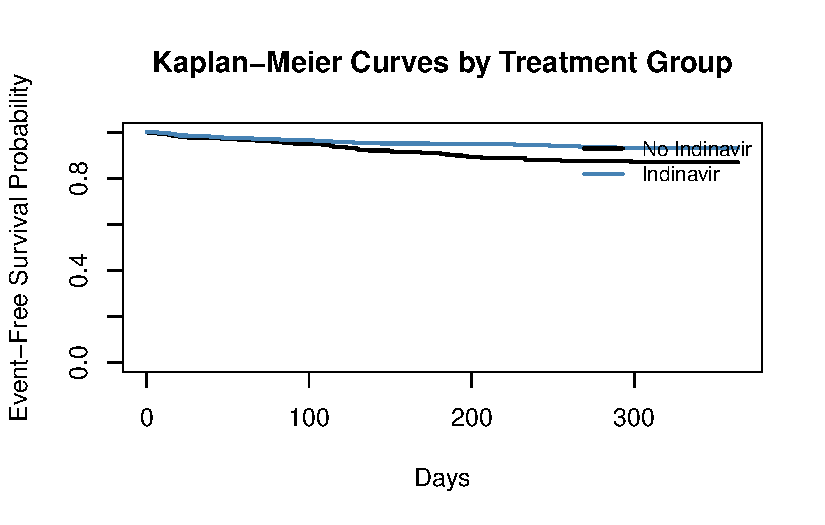
\includegraphics[width=0.8\linewidth,height=\textheight,keepaspectratio]{Math261B_Final_Paper_v1_files/figure-pdf/fig-km-plot-1.pdf}

}

\caption{\label{fig-km-plot}Kaplan-Meier survival curves for Indinavir
versus No Indinavir treatment groups.}

\end{figure}%

To estimate the treatment effect while adjusting for patient
characteristics, we fit a Cox proportional hazards model. The model
includes treatment assignment, baseline CD4 count, age, Karnofsky
performance score, months of prior ZDV use, and CD4 count stratum. The
full regression results are shown in Table~\ref{tbl-whole-group}.

\begin{longtable}[]{@{}
  >{\raggedright\arraybackslash}p{(\linewidth - 8\tabcolsep) * \real{0.4872}}
  >{\raggedleft\arraybackslash}p{(\linewidth - 8\tabcolsep) * \real{0.0769}}
  >{\raggedleft\arraybackslash}p{(\linewidth - 8\tabcolsep) * \real{0.1667}}
  >{\raggedleft\arraybackslash}p{(\linewidth - 8\tabcolsep) * \real{0.1667}}
  >{\raggedleft\arraybackslash}p{(\linewidth - 8\tabcolsep) * \real{0.1026}}@{}}
\caption{Whole-Group Baseline Cox Model --- Hazard
Ratios}\label{tbl-whole-group}\tabularnewline
\toprule\noalign{}
\begin{minipage}[b]{\linewidth}\raggedright
Covariate
\end{minipage} & \begin{minipage}[b]{\linewidth}\raggedleft
HR
\end{minipage} & \begin{minipage}[b]{\linewidth}\raggedleft
95\% CI Lower
\end{minipage} & \begin{minipage}[b]{\linewidth}\raggedleft
95\% CI Upper
\end{minipage} & \begin{minipage}[b]{\linewidth}\raggedleft
p-value
\end{minipage} \\
\midrule\noalign{}
\endfirsthead
\toprule\noalign{}
\begin{minipage}[b]{\linewidth}\raggedright
Covariate
\end{minipage} & \begin{minipage}[b]{\linewidth}\raggedleft
HR
\end{minipage} & \begin{minipage}[b]{\linewidth}\raggedleft
95\% CI Lower
\end{minipage} & \begin{minipage}[b]{\linewidth}\raggedleft
95\% CI Upper
\end{minipage} & \begin{minipage}[b]{\linewidth}\raggedleft
p-value
\end{minipage} \\
\midrule\noalign{}
\endhead
\bottomrule\noalign{}
\endlastfoot
Treatment: Indinavir vs.~No Indinavir & 0.517 & 0.339 & 0.788 & 0.002 \\
Age & 1.022 & 1.000 & 1.045 & 0.054 \\
Baseline CD4 & 0.985 & 0.978 & 0.993 & 0.000 \\
Karnofsky Score & 0.948 & 0.926 & 0.970 & 0.000 \\
Prior ZDV Use & 1.000 & 0.992 & 1.007 & 0.925 \\
CD4 Stratum & 1.012 & 0.517 & 1.984 & 0.971 \\
\end{longtable}

The estimated hazard ratio for treatment is HR = 0.517. This means that
at any point in time during follow-up, patients receiving indinavir had
approximately half the hazard of experiencing an AIDS-defining event or
death compared to the control group, after adjusting for other
covariates. This is consistent with the original findings of Hammer et
al.~(1997). A log-rank test confirms overall treatment group separation,
with a chi-square statistic of 10.545 on 1 degree of freedom (p =
0.0012), indicating that the difference in event timing between the two
treatment groups is statistically significant.

\subsection{Sex Subgroup}\label{sex-subgroup}

To examine whether the treatment effect differed between men and women,
we fit two models. The first is a baseline model that includes sex as a
fixed covariate alongside treatment. The second is a full model that
adds a treatment-by-sex interaction term. A likelihood ratio test
compares the two models. We then fit separate Cox models for females and
males to estimate sex-specific hazard ratios.

The sex baseline and full interaction models are reported in Appendix
Tables A1 and A2. The baseline treatment hazard ratio remains
approximately unchanged at 0.517, and the coefficient for sex is not
statistically significant, indicating that sex does not meaningfully
confound the overall treatment effect. In the full interaction model,
the hazard ratio for treatment among females, the reference group, is
0.46. The interaction hazard ratio is 2.034, but the likelihood ratio
test yields a p-value of 0.2187, so adding the interaction term does not
significantly improve model fit. We cannot conclude that sex modifies
the treatment effect.

The sex-specific models yield a hazard ratio of 0.459 for female
participants and 1.101 for male participants. With only 15 events among
male participants across 200 enrolled individuals, the Cox model for
males is severely underpowered estimated treatment effect should be
interpreted with caution.

\subsection{Race/Ethnicity Subgroup}\label{raceethnicity-subgroup}

To examine whether the treatment effect differed across race and
ethnicity groups, we fit a baseline model that includes race/ethnicity
as a fixed covariate and a full model that adds
treatment-by-race/ethnicity interaction terms. Race/ethnicity is coded
as a five-level factor with White non-Hispanic participants as the
reference group. We then fit separate Cox models within each
race/ethnicity group to estimate group-specific hazard ratios.

The baseline model yields a treatment hazard ratio of 0.526, indicating
that after adjusting for race/ethnicity, patients receiving indinavir
had approximately 47\% lower hazard of AIDS-defining events or death.
The full race/ethnicity interaction model is reported in Appendix Table
A3. The interaction terms for Black, Hispanic, and Other are not
statistically significant, providing no clear evidence that the
treatment effect differs across these groups. The interaction term for
the Asian/Pacific Islander group has a p-value of 0.033, but the
confidence interval is extremely wide because there were only 3 events
in that subgroup. The likelihood ratio test gives a chi-square statistic
of 8.326 with 4 degrees of freedom (p = 0.0803), so we cannot conclude
that race/ethnicity modifies the treatment effect.

\subsection{Summary of All Effect
Sizes}\label{summary-of-all-effect-sizes}

Table~\ref{tbl-summary} presents all hazard ratio estimates across the
whole group, sex, and race/ethnicity analyses. Estimates are stable for
the overall group and larger subgroups but become unreliable as event
counts fall. For Asian/PI and Other, the estimates are essentially
uninformative. An HR less than 1 indicates that indinavir-containing
therapy reduces the hazard of AIDS-defining events or death relative to
nucleoside-only therapy.

\begin{longtable}[]{@{}
  >{\raggedright\arraybackslash}p{(\linewidth - 14\tabcolsep) * \real{0.1412}}
  >{\raggedright\arraybackslash}p{(\linewidth - 14\tabcolsep) * \real{0.2118}}
  >{\raggedright\arraybackslash}p{(\linewidth - 14\tabcolsep) * \real{0.1059}}
  >{\raggedright\arraybackslash}p{(\linewidth - 14\tabcolsep) * \real{0.0588}}
  >{\raggedleft\arraybackslash}p{(\linewidth - 14\tabcolsep) * \real{0.0824}}
  >{\raggedleft\arraybackslash}p{(\linewidth - 14\tabcolsep) * \real{0.0941}}
  >{\raggedleft\arraybackslash}p{(\linewidth - 14\tabcolsep) * \real{0.1529}}
  >{\raggedleft\arraybackslash}p{(\linewidth - 14\tabcolsep) * \real{0.1529}}@{}}
\caption{Summary of Treatment Effect Sizes Across All
Analyses}\label{tbl-summary}\tabularnewline
\toprule\noalign{}
\begin{minipage}[b]{\linewidth}\raggedright
Analysis
\end{minipage} & \begin{minipage}[b]{\linewidth}\raggedright
Model
\end{minipage} & \begin{minipage}[b]{\linewidth}\raggedright
Subgroup
\end{minipage} & \begin{minipage}[b]{\linewidth}\raggedright
n
\end{minipage} & \begin{minipage}[b]{\linewidth}\raggedleft
Events
\end{minipage} & \begin{minipage}[b]{\linewidth}\raggedleft
HR
\end{minipage} & \begin{minipage}[b]{\linewidth}\raggedleft
95\% CI Lower
\end{minipage} & \begin{minipage}[b]{\linewidth}\raggedleft
95\% CI Upper
\end{minipage} \\
\midrule\noalign{}
\endfirsthead
\toprule\noalign{}
\begin{minipage}[b]{\linewidth}\raggedright
Analysis
\end{minipage} & \begin{minipage}[b]{\linewidth}\raggedright
Model
\end{minipage} & \begin{minipage}[b]{\linewidth}\raggedright
Subgroup
\end{minipage} & \begin{minipage}[b]{\linewidth}\raggedright
n
\end{minipage} & \begin{minipage}[b]{\linewidth}\raggedleft
Events
\end{minipage} & \begin{minipage}[b]{\linewidth}\raggedleft
HR
\end{minipage} & \begin{minipage}[b]{\linewidth}\raggedleft
95\% CI Lower
\end{minipage} & \begin{minipage}[b]{\linewidth}\raggedleft
95\% CI Upper
\end{minipage} \\
\midrule\noalign{}
\endhead
\bottomrule\noalign{}
\endlastfoot
Whole Group & Baseline & All & 1151 & 96 & 0.517 & 0.339 & 0.788 \\
Sex & Baseline (pooled) & All & 1151 & 96 & 0.517 & 0.339 & 0.789 \\
Sex & Stratum-specific & Female & 951 & 81 & 0.459 & 0.288 & 0.732 \\
Sex & Stratum-specific & Male & 200 & 15 & 1.101 & 0.393 & 3.087 \\
Race & Baseline (pooled) & All & 1151 & 96 & 0.526 & 0.344 & 0.805 \\
Race & Stratum-specific & White & 596 & 51 & 0.539 & 0.303 & 0.960 \\
Race & Stratum-specific & Black & 327 & 21 & 0.287 & 0.104 & 0.794 \\
Race & Stratum-specific & Hispanic & 203 & 20 & 0.628 & 0.246 & 1.602 \\
Race & Stratum-specific & Asian/PI & 14 & 3 & 0.068 & 0.000 & Inf \\
Race & Stratum-specific & Other & 11 & 1 & 237.311 & 0.000 & Inf \\
\end{longtable}

\subsection{Power Analysis}\label{power-analysis}

Before estimating sample sizes for future studies, we calculated the
observed power of the ACTG 320 analyses for the overall population and
each subgroup. Power was estimated assuming equal allocation between
treatment and control groups. To account for multiple hypothesis
testing, we used a Bonferroni-adjusted significance level of
\(\alpha = 0.025\) for each interaction test. This adjustment controls
the family-wise error rate across the two primary subgroup comparisons
(sex and race/ethnicity), ensuring that the overall probability of a
Type I error remains bounded at 0.05.

The observed power estimates are shown in
Table~\ref{tbl-observed-power}. Only the overall group and the female
subgroup exceeded the 80\% power threshold. All other subgroups fell
below it, and for the male, Asian/Pacific Islander, and Other subgroups,
the underlying hazard ratio estimates are themselves too unstable to
produce meaningful power calculations.

\begin{longtable}[]{@{}
  >{\raggedright\arraybackslash}p{(\linewidth - 14\tabcolsep) * \real{0.1667}}
  >{\raggedright\arraybackslash}p{(\linewidth - 14\tabcolsep) * \real{0.1000}}
  >{\raggedleft\arraybackslash}p{(\linewidth - 14\tabcolsep) * \real{0.0556}}
  >{\raggedleft\arraybackslash}p{(\linewidth - 14\tabcolsep) * \real{0.0778}}
  >{\raggedleft\arraybackslash}p{(\linewidth - 14\tabcolsep) * \real{0.1333}}
  >{\raggedleft\arraybackslash}p{(\linewidth - 14\tabcolsep) * \real{0.1222}}
  >{\raggedleft\arraybackslash}p{(\linewidth - 14\tabcolsep) * \real{0.1667}}
  >{\raggedright\arraybackslash}p{(\linewidth - 14\tabcolsep) * \real{0.1778}}@{}}
\caption{Initial Observed Power by Overall Group and
Subgroup}\label{tbl-observed-power}\tabularnewline
\toprule\noalign{}
\begin{minipage}[b]{\linewidth}\raggedright
Analysis
\end{minipage} & \begin{minipage}[b]{\linewidth}\raggedright
Subgroup
\end{minipage} & \begin{minipage}[b]{\linewidth}\raggedleft
n
\end{minipage} & \begin{minipage}[b]{\linewidth}\raggedleft
Events
\end{minipage} & \begin{minipage}[b]{\linewidth}\raggedleft
Observed HR
\end{minipage} & \begin{minipage}[b]{\linewidth}\raggedleft
Event Rate
\end{minipage} & \begin{minipage}[b]{\linewidth}\raggedleft
Observed Power
\end{minipage} & \begin{minipage}[b]{\linewidth}\raggedright
Interpretation
\end{minipage} \\
\midrule\noalign{}
\endfirsthead
\toprule\noalign{}
\begin{minipage}[b]{\linewidth}\raggedright
Analysis
\end{minipage} & \begin{minipage}[b]{\linewidth}\raggedright
Subgroup
\end{minipage} & \begin{minipage}[b]{\linewidth}\raggedleft
n
\end{minipage} & \begin{minipage}[b]{\linewidth}\raggedleft
Events
\end{minipage} & \begin{minipage}[b]{\linewidth}\raggedleft
Observed HR
\end{minipage} & \begin{minipage}[b]{\linewidth}\raggedleft
Event Rate
\end{minipage} & \begin{minipage}[b]{\linewidth}\raggedleft
Observed Power
\end{minipage} & \begin{minipage}[b]{\linewidth}\raggedright
Interpretation
\end{minipage} \\
\midrule\noalign{}
\endhead
\bottomrule\noalign{}
\endlastfoot
Whole Group & All & 1151 & 96 & 0.517 & 0.083 & 0.839 & At or above
80\% \\
Sex & Female & 951 & 81 & 0.459 & 0.085 & 0.897 & At or above 80\% \\
Sex & Male & 200 & 15 & 1.101 & 0.075 & 0.020 & Below 80\% \\
Race/Ethnicity & White & 596 & 51 & 0.539 & 0.086 & 0.486 & Below
80\% \\
Race/Ethnicity & Black & 327 & 21 & 0.287 & 0.064 & 0.732 & Below
80\% \\
Race/Ethnicity & Hispanic & 203 & 20 & 0.628 & 0.099 & 0.115 & Below
80\% \\
Race/Ethnicity & Asian/PI & 14 & 3 & 0.068 & 0.214 & 0.535 & Below
80\% \\
Race/Ethnicity & Other & 11 & 1 & 237.311 & 0.091 & 0.689 & Below
80\% \\
\end{longtable}

Detailed sample size calculations are provided in Appendix Tables
A4--A6. For subgroups with more stable hazard ratio estimates, required
sample sizes were calculated at 80\%, 85\%, 90\%, and 95\% power. For
male, Asian/PI, and Other subgroups, where the observed hazard ratios
were unstable, required sample sizes were calculated across assumed
hazard ratios from 0.50 to 0.90. The Hispanic subgroup stands out as the
only stable subgroup that was underpowered in ACTG 320, requiring
approximately 447 participants to achieve 80\% power compared to the 203
enrolled.

\begin{figure}

\centering{

\pandocbounded{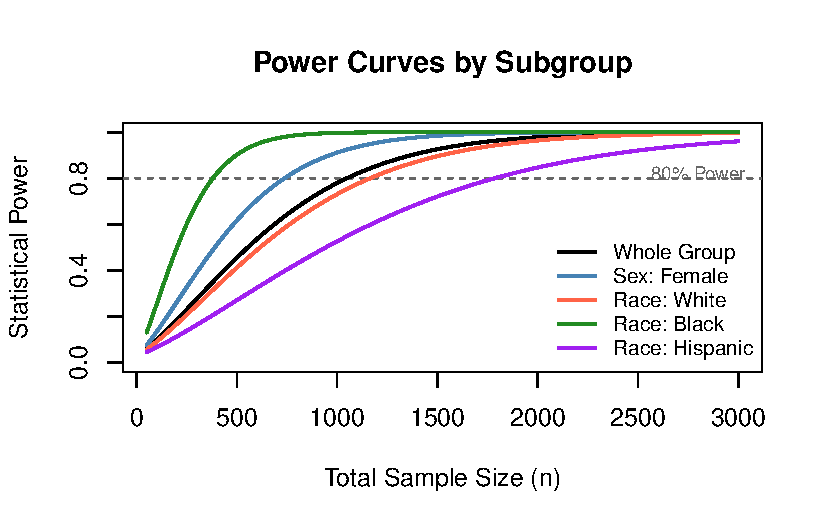
\includegraphics[keepaspectratio]{Math261B_Final_Paper_v1_files/figure-pdf/fig-power-curves-1.pdf}}

}

\caption{\label{fig-power-curves}Power curves showing achieved power as
a function of sample size for each reliable subgroup, with the 80\%
power threshold shown.}

\end{figure}%

\begin{longtable}[]{@{}
  >{\raggedright\arraybackslash}p{(\linewidth - 8\tabcolsep) * \real{0.1899}}
  >{\raggedleft\arraybackslash}p{(\linewidth - 8\tabcolsep) * \real{0.1519}}
  >{\raggedleft\arraybackslash}p{(\linewidth - 8\tabcolsep) * \real{0.1392}}
  >{\raggedleft\arraybackslash}p{(\linewidth - 8\tabcolsep) * \real{0.3165}}
  >{\raggedright\arraybackslash}p{(\linewidth - 8\tabcolsep) * \real{0.2025}}@{}}
\caption{Adequacy of ACTG 320 Sample Sizes for 80\%
Power}\label{tbl-power-adequacy}\tabularnewline
\toprule\noalign{}
\begin{minipage}[b]{\linewidth}\raggedright
Subgroup
\end{minipage} & \begin{minipage}[b]{\linewidth}\raggedleft
Observed HR
\end{minipage} & \begin{minipage}[b]{\linewidth}\raggedleft
ACTG 320 n
\end{minipage} & \begin{minipage}[b]{\linewidth}\raggedleft
Required n for 80\% Power
\end{minipage} & \begin{minipage}[b]{\linewidth}\raggedright
ACTG 320 Status
\end{minipage} \\
\midrule\noalign{}
\endfirsthead
\toprule\noalign{}
\begin{minipage}[b]{\linewidth}\raggedright
Subgroup
\end{minipage} & \begin{minipage}[b]{\linewidth}\raggedleft
Observed HR
\end{minipage} & \begin{minipage}[b]{\linewidth}\raggedleft
ACTG 320 n
\end{minipage} & \begin{minipage}[b]{\linewidth}\raggedleft
Required n for 80\% Power
\end{minipage} & \begin{minipage}[b]{\linewidth}\raggedright
ACTG 320 Status
\end{minipage} \\
\midrule\noalign{}
\endhead
\bottomrule\noalign{}
\endlastfoot
Whole Group & 0.517 & 1151 & 264 & Adequate \\
Sex: Female & 0.459 & 951 & 188 & Adequate \\
Race: White & 0.539 & 596 & 293 & Adequate \\
Race: Black & 0.287 & 327 & 109 & Adequate \\
Race: Hispanic & 0.628 & 203 & 447 & Underpowered \\
\end{longtable}

\section{Discussion}\label{sec-discussion}

This paper reanalyzed the ACTG 320 clinical trial {[}@Hammer1997{]} to
evaluate how demographic subgroup representation and observed event
counts affect statistical power in time-to-event analyses. We
successfully replicated the primary treatment effect:
indinavir-containing combination therapy reduced the hazard of
progression to AIDS or death by approximately 48\% relative to the
control regimen (HR = 0.517), consistent with the original findings.
This result was stable across all baseline model specifications and was
statistically significant (log-rank p = 0.0012), confirming that the
overall study had adequate power for its intended purpose.

Subgroup analyses revealed a more complicated picture. We did not detect
statistically significant treatment-by-sex or
treatment-by-race/ethnicity interaction effects. The data do not provide
evidence that indinavir's benefit differed across demographic groups.
However, this result is not evidence of homogeneous treatment effects.
The power analysis demonstrates that most subgroups were never in a
position to detect meaningful differences. The male stratum contributed
only 15 events across 200 enrolled participants, leaving the
stratum-specific Cox model severely underpowered and its hazard ratio
estimate (HR = 1.101) unreliable. The Asian/Pacific Islander and Other
race subgroups contributed 3 and 1 events, respectively, making their
estimates entirely uninformative. Even among the more stable subgroups,
only the overall group and the female subgroup exceeded the 80\% power
threshold at the observed effect sizes. The Hispanic subgroup enrolled
203 participants but remained underpowered because its low event count
(20 events) was insufficient to detect a moderate treatment effect. It
would require enrollment of approximately 447 participants to achieve
80\% power.

The central lesson of the power analysis is that observed events, not
enrollment, determine power in survival studies. This distinction is not
always apparent in the clinical trial literature. Representation is
often discussed in terms of enrollment proportions rather than
event-driven inferential capacity. A subgroup that is nominally
represented in a trial may still contribute too few events to support
any meaningful conclusion about treatment heterogeneity. The results
here quantify that gap explicitly: for the underpowered subgroups,
achieving 80\% power would require enrollment increases ranging from
modest (approximately 94 participants for Asian/PI assuming HR = 0.50)
to very large (over 11,000 for male participants assuming HR = 0.90).
These figures illustrate that when the true treatment effect is small or
moderate, the sample size requirements for subgroup inference can be
prohibitive within a single trial.

\subsection{Limitations}\label{limitations}

This analysis had several limitations. First, the analysis relies on
secondary use of a publicly available dataset and can only use variables
included in the public data release. Secondary endpoints from the
original trial, CD4 cell count trajectories, and HIV-1 RNA
concentrations, are not available, limiting this reanalysis to the
primary time-to-event outcome. Second, the total number of primary
endpoint events was small (96 across 1,151 participants), which
constrains the precision of all subgroup analyses regardless of modeling
approach. Third, the power calculations rely on asymptotic
approximations under the Cox proportional hazards framework and assume
that hazard ratios remain proportional over the follow-up period. This
assumption may not hold in all subgroups, given the sparse event counts.
Fourth, the race/ethnicity variable in the available dataset contains
only five levels; the American Indian/Alaska Native category described
in the original trial protocol is absent from the public data. The
ethnicity analysis has less coverage than the original design intended.
Finally, post-hoc power estimates for the most underpowered subgroups,
male, Asian/PI, and Other, should be treated as descriptive only because
the underlying hazard ratio estimates driving those calculations are
themselves unstable.

\subsection{Implications and Future
Research}\label{implications-and-future-research}

The findings of this paper have direct implications for the design of
future clinical trials where subgroup-specific inference is a scientific
objective. Trials powered only for overall treatment comparisons are
structurally unable to detect differential treatment responses in
underrepresented demographic groups, not because those differences do
not exist, but because the study lacks the power to detect them. This
problem is particularly consequential for historically underrepresented
populations in clinical research, who may face distinct biological,
pharmacological, or social determinants of treatment response. As
@Khan2020 and @Poon2013 document, this pattern is not specific to HIV
trials; it is a persistent feature of pivotal drug development across
therapeutic areas.

Practical solutions exist but require intentional trial design.
Prospective enrollment targets for key demographic subgroups, set based
on anticipated event rates and minimum detectable effect sizes rather
than proportional representation alone, would ensure that subgroup
analyses are interpretable rather than merely exploratory. Extending
follow-up duration increases event accrual without requiring additional
enrollment, which may be a cost-effective strategy to improve subgroup
power in trials with low overall event rates. Another option is adaptive
event-driven designs that trigger subgroup analyses only after reaching
subgroup-specific event thresholds. For situations where no single trial
can achieve adequate subgroup enrollment, Bayesian hierarchical models
that borrow information across subgroups under assumptions of partial
exchangeability, and pooled meta-analytic frameworks across multiple
trials, may provide the inferential capacity that individual studies
cannot. Future methodological work should evaluate the performance of
these approaches specifically under the sparse-event subgroup conditions
illustrated here.

\newpage
\appendix

\section{Supplemental Tables}\label{supplemental-tables}

\subsection{Supplemental Sex Model
Tables}\label{supplemental-sex-model-tables}

\begin{longtable}[]{@{}lrrrr@{}}
\caption{Appendix Table A1. Sex Baseline Cox Model --- Hazard
Ratios}\label{tbl-app-sex-baseline}\tabularnewline
\toprule\noalign{}
Covariate & HR & 95\% CI Lower & 95\% CI Upper & p-value \\
\midrule\noalign{}
\endfirsthead
\toprule\noalign{}
Covariate & HR & 95\% CI Lower & 95\% CI Upper & p-value \\
\midrule\noalign{}
\endhead
\bottomrule\noalign{}
\endlastfoot
Treatment (IDV vs no IDV) & 0.517 & 0.339 & 0.789 & 0.002 \\
Sex (Male vs Female) & 1.122 & 0.643 & 1.957 & 0.685 \\
Age & 1.023 & 1.000 & 1.046 & 0.050 \\
Baseline CD4 & 0.985 & 0.978 & 0.993 & 0.000 \\
Karnofsky Score & 0.948 & 0.926 & 0.970 & 0.000 \\
Prior ZDV Use & 1.000 & 0.992 & 1.007 & 0.926 \\
CD4 Stratum & 1.013 & 0.517 & 1.985 & 0.970 \\
\end{longtable}

\begin{longtable}[]{@{}lrrrr@{}}
\caption{Appendix Table A2. Sex Full Cox Model with Interaction ---
Hazard Ratios}\label{tbl-app-sex-full}\tabularnewline
\toprule\noalign{}
Covariate & HR & 95\% CI Lower & 95\% CI Upper & p-value \\
\midrule\noalign{}
\endfirsthead
\toprule\noalign{}
Covariate & HR & 95\% CI Lower & 95\% CI Upper & p-value \\
\midrule\noalign{}
\endhead
\bottomrule\noalign{}
\endlastfoot
Treatment (IDV vs no IDV) & 0.460 & 0.288 & 0.734 & 0.001 \\
Sex (Male vs Female) & 0.854 & 0.405 & 1.801 & 0.679 \\
Age & 1.023 & 1.000 & 1.046 & 0.050 \\
Baseline CD4 & 0.985 & 0.978 & 0.993 & 0.000 \\
Karnofsky Score & 0.947 & 0.925 & 0.969 & 0.000 \\
Prior ZDV Use & 0.999 & 0.992 & 1.007 & 0.865 \\
CD4 Stratum & 1.011 & 0.516 & 1.978 & 0.975 \\
Treatment x Sex & 2.034 & 0.663 & 6.238 & 0.214 \\
\end{longtable}

\subsection{Supplemental Race/Ethnicity Model
Table}\label{supplemental-raceethnicity-model-table}

\begin{longtable}[]{@{}
  >{\raggedright\arraybackslash}p{(\linewidth - 8\tabcolsep) * \real{0.3881}}
  >{\raggedleft\arraybackslash}p{(\linewidth - 8\tabcolsep) * \real{0.1045}}
  >{\raggedleft\arraybackslash}p{(\linewidth - 8\tabcolsep) * \real{0.1940}}
  >{\raggedleft\arraybackslash}p{(\linewidth - 8\tabcolsep) * \real{0.1940}}
  >{\raggedleft\arraybackslash}p{(\linewidth - 8\tabcolsep) * \real{0.1194}}@{}}
\caption{Appendix Table A3. Race Full Cox Model with Interaction ---
Hazard Ratios}\label{tbl-app-race-full}\tabularnewline
\toprule\noalign{}
\begin{minipage}[b]{\linewidth}\raggedright
Covariate
\end{minipage} & \begin{minipage}[b]{\linewidth}\raggedleft
HR
\end{minipage} & \begin{minipage}[b]{\linewidth}\raggedleft
95\% CI Lower
\end{minipage} & \begin{minipage}[b]{\linewidth}\raggedleft
95\% CI Upper
\end{minipage} & \begin{minipage}[b]{\linewidth}\raggedleft
p-value
\end{minipage} \\
\midrule\noalign{}
\endfirsthead
\toprule\noalign{}
\begin{minipage}[b]{\linewidth}\raggedright
Covariate
\end{minipage} & \begin{minipage}[b]{\linewidth}\raggedleft
HR
\end{minipage} & \begin{minipage}[b]{\linewidth}\raggedleft
95\% CI Lower
\end{minipage} & \begin{minipage}[b]{\linewidth}\raggedleft
95\% CI Upper
\end{minipage} & \begin{minipage}[b]{\linewidth}\raggedleft
p-value
\end{minipage} \\
\midrule\noalign{}
\endhead
\bottomrule\noalign{}
\endlastfoot
Treatment (IDV vs no IDV) & 0.534 & 0.302 & 0.946 & 0.032 \\
Race: Black (vs White) & 0.794 & 0.432 & 1.457 & 0.456 \\
Race: Hispanic (vs White) & 1.002 & 0.524 & 1.914 & 0.995 \\
Race: Asian/PI (vs White) & 0.860 & 0.117 & 6.317 & 0.882 \\
Race: Other (vs White) & 2.831 & 0.378 & 21.227 & 0.311 \\
Age & 1.024 & 1.001 & 1.048 & 0.038 \\
Baseline CD4 & 0.985 & 0.978 & 0.993 & 0.000 \\
Karnofsky Score & 0.948 & 0.927 & 0.971 & 0.000 \\
Prior ZDV Use & 0.997 & 0.989 & 1.005 & 0.467 \\
CD4 Stratum & 1.010 & 0.513 & 1.986 & 0.978 \\
Treatment x Black & 0.591 & 0.185 & 1.883 & 0.373 \\
Treatment x Hispanic & 1.249 & 0.422 & 3.698 & 0.687 \\
Treatment x Asian/PI & 15.514 & 1.244 & 193.477 & 0.033 \\
Treatment x Other & 0.000 & 0.000 & Inf & 0.993 \\
\end{longtable}

\subsection{Supplemental Power Analysis
Tables}\label{supplemental-power-analysis-tables}

\begin{longtable}[]{@{}
  >{\raggedright\arraybackslash}p{(\linewidth - 16\tabcolsep) * \real{0.1685}}
  >{\raggedleft\arraybackslash}p{(\linewidth - 16\tabcolsep) * \real{0.1348}}
  >{\raggedleft\arraybackslash}p{(\linewidth - 16\tabcolsep) * \real{0.0787}}
  >{\raggedleft\arraybackslash}p{(\linewidth - 16\tabcolsep) * \real{0.1348}}
  >{\raggedleft\arraybackslash}p{(\linewidth - 16\tabcolsep) * \real{0.1236}}
  >{\raggedleft\arraybackslash}p{(\linewidth - 16\tabcolsep) * \real{0.0899}}
  >{\raggedleft\arraybackslash}p{(\linewidth - 16\tabcolsep) * \real{0.0899}}
  >{\raggedleft\arraybackslash}p{(\linewidth - 16\tabcolsep) * \real{0.0899}}
  >{\raggedleft\arraybackslash}p{(\linewidth - 16\tabcolsep) * \real{0.0899}}@{}}
\caption{Appendix Table A4. Required Sample Sizes by Subgroup and Power
Level (\(\alpha\) = 0.025)}\label{tbl-app-power-reliable}\tabularnewline
\toprule\noalign{}
\begin{minipage}[b]{\linewidth}\raggedright
Subgroup
\end{minipage} & \begin{minipage}[b]{\linewidth}\raggedleft
Observed HR
\end{minipage} & \begin{minipage}[b]{\linewidth}\raggedleft
Obs. n
\end{minipage} & \begin{minipage}[b]{\linewidth}\raggedleft
Obs. Events
\end{minipage} & \begin{minipage}[b]{\linewidth}\raggedleft
Event Rate
\end{minipage} & \begin{minipage}[b]{\linewidth}\raggedleft
n (80\%)
\end{minipage} & \begin{minipage}[b]{\linewidth}\raggedleft
n (85\%)
\end{minipage} & \begin{minipage}[b]{\linewidth}\raggedleft
n (90\%)
\end{minipage} & \begin{minipage}[b]{\linewidth}\raggedleft
n (95\%)
\end{minipage} \\
\midrule\noalign{}
\endfirsthead
\toprule\noalign{}
\begin{minipage}[b]{\linewidth}\raggedright
Subgroup
\end{minipage} & \begin{minipage}[b]{\linewidth}\raggedleft
Observed HR
\end{minipage} & \begin{minipage}[b]{\linewidth}\raggedleft
Obs. n
\end{minipage} & \begin{minipage}[b]{\linewidth}\raggedleft
Obs. Events
\end{minipage} & \begin{minipage}[b]{\linewidth}\raggedleft
Event Rate
\end{minipage} & \begin{minipage}[b]{\linewidth}\raggedleft
n (80\%)
\end{minipage} & \begin{minipage}[b]{\linewidth}\raggedleft
n (85\%)
\end{minipage} & \begin{minipage}[b]{\linewidth}\raggedleft
n (90\%)
\end{minipage} & \begin{minipage}[b]{\linewidth}\raggedleft
n (95\%)
\end{minipage} \\
\midrule\noalign{}
\endhead
\bottomrule\noalign{}
\endlastfoot
Whole Group & 0.517 & 1151 & 96 & 0.083 & 264 & 300 & 348 & 420 \\
Sex: Female & 0.459 & 951 & 81 & 0.085 & 188 & 212 & 247 & 294 \\
Race: White & 0.539 & 596 & 51 & 0.086 & 293 & 339 & 386 & 468 \\
Race: Black & 0.287 & 327 & 21 & 0.064 & 109 & 109 & 125 & 156 \\
Race: Hispanic & 0.628 & 203 & 20 & 0.099 & 447 & 508 & 589 & 711 \\
\end{longtable}

\begin{longtable}[]{@{}
  >{\raggedright\arraybackslash}p{(\linewidth - 6\tabcolsep) * \real{0.2113}}
  >{\raggedright\arraybackslash}p{(\linewidth - 6\tabcolsep) * \real{0.1549}}
  >{\raggedleft\arraybackslash}p{(\linewidth - 6\tabcolsep) * \real{0.2817}}
  >{\raggedleft\arraybackslash}p{(\linewidth - 6\tabcolsep) * \real{0.3521}}@{}}
\caption{Appendix Table A5. Required Sample Sizes for 80\% Power Across
Assumed Hazard Ratios}\label{tbl-app-power-underpowered}\tabularnewline
\toprule\noalign{}
\begin{minipage}[b]{\linewidth}\raggedright
Subgroup
\end{minipage} & \begin{minipage}[b]{\linewidth}\raggedright
Assumed HR
\end{minipage} & \begin{minipage}[b]{\linewidth}\raggedleft
Observed Event Rate
\end{minipage} & \begin{minipage}[b]{\linewidth}\raggedleft
Required n for 80\% Power
\end{minipage} \\
\midrule\noalign{}
\endfirsthead
\toprule\noalign{}
\begin{minipage}[b]{\linewidth}\raggedright
Subgroup
\end{minipage} & \begin{minipage}[b]{\linewidth}\raggedright
Assumed HR
\end{minipage} & \begin{minipage}[b]{\linewidth}\raggedleft
Observed Event Rate
\end{minipage} & \begin{minipage}[b]{\linewidth}\raggedleft
Required n for 80\% Power
\end{minipage} \\
\midrule\noalign{}
\endhead
\bottomrule\noalign{}
\endlastfoot
Sex: Male & 0.5 & 0.075 & 267 \\
Sex: Male & 0.6 & 0.075 & 494 \\
Sex: Male & 0.7 & 0.075 & 1000 \\
Sex: Male & 0.8 & 0.075 & 2547 \\
Sex: Male & 0.9 & 0.075 & 11427 \\
Race: Asian/PI & 0.5 & 0.214 & 94 \\
Race: Asian/PI & 0.6 & 0.214 & 173 \\
Race: Asian/PI & 0.7 & 0.214 & 350 \\
Race: Asian/PI & 0.8 & 0.214 & 892 \\
Race: Asian/PI & 0.9 & 0.214 & 4000 \\
Race: Other & 0.5 & 0.091 & 220 \\
Race: Other & 0.6 & 0.091 & 407 \\
Race: Other & 0.7 & 0.091 & 825 \\
Race: Other & 0.8 & 0.091 & 2101 \\
Race: Other & 0.9 & 0.091 & 9427 \\
\end{longtable}

\begin{longtable}[]{@{}
  >{\raggedright\arraybackslash}p{(\linewidth - 8\tabcolsep) * \real{0.1613}}
  >{\raggedleft\arraybackslash}p{(\linewidth - 8\tabcolsep) * \real{0.1290}}
  >{\raggedleft\arraybackslash}p{(\linewidth - 8\tabcolsep) * \real{0.1183}}
  >{\raggedleft\arraybackslash}p{(\linewidth - 8\tabcolsep) * \real{0.3226}}
  >{\raggedleft\arraybackslash}p{(\linewidth - 8\tabcolsep) * \real{0.2688}}@{}}
\caption{Appendix Table A6. Required Events and Sample Sizes for 80\%
Power}\label{tbl-app-power-events}\tabularnewline
\toprule\noalign{}
\begin{minipage}[b]{\linewidth}\raggedright
Subgroup
\end{minipage} & \begin{minipage}[b]{\linewidth}\raggedleft
Observed HR
\end{minipage} & \begin{minipage}[b]{\linewidth}\raggedleft
Event Rate
\end{minipage} & \begin{minipage}[b]{\linewidth}\raggedleft
Events Required for 80\% Power
\end{minipage} & \begin{minipage}[b]{\linewidth}\raggedleft
Required n for 80\% Power
\end{minipage} \\
\midrule\noalign{}
\endfirsthead
\toprule\noalign{}
\begin{minipage}[b]{\linewidth}\raggedright
Subgroup
\end{minipage} & \begin{minipage}[b]{\linewidth}\raggedleft
Observed HR
\end{minipage} & \begin{minipage}[b]{\linewidth}\raggedleft
Event Rate
\end{minipage} & \begin{minipage}[b]{\linewidth}\raggedleft
Events Required for 80\% Power
\end{minipage} & \begin{minipage}[b]{\linewidth}\raggedleft
Required n for 80\% Power
\end{minipage} \\
\midrule\noalign{}
\endhead
\bottomrule\noalign{}
\endlastfoot
Whole Group & 0.517 & 0.083 & 22 & 264 \\
Sex: Female & 0.459 & 0.085 & 16 & 188 \\
Race: White & 0.539 & 0.086 & 25 & 293 \\
Race: Black & 0.287 & 0.064 & 7 & 109 \\
Race: Hispanic & 0.628 & 0.099 & 44 & 447 \\
\end{longtable}

\section*{References}\label{references}
\addcontentsline{toc}{section}{References}

\phantomsection\label{refs}
\begin{CSLReferences}{1}{0}
\bibitem[\citeproctext]{ref-Eshera2015}
Eshera, N., H. Itana, L. Zhang, G. Soon, and E. Fadiran. 2015.
{``Demographics of Clinical Trial Participants in Pivotal Trials for New
Molecular Entity Drugs.''} \emph{The American Journal of Therapeutics}
22 (6): 435--55.

\bibitem[\citeproctext]{ref-Hammer1997}
Hammer, Scott M., Kathleen E. Squires, Michael D. Hughes, Janet M.
Grimes, Lisa M. Demeter, Judith S. Currier, Joseph J. Eron, et al. 1997.
{``A Controlled Trial of Two Nucleoside Analogues Plus Indinavir in
Persons with Human Immunodeficiency Virus Infection and {CD4} Cell
Counts of 200 Per Cubic Millimeter or Less.''} \emph{New England Journal
of Medicine} 337 (11): 725--33.
\url{https://doi.org/10.1056/NEJM199709113371101}.

\bibitem[\citeproctext]{ref-Khan2020}
Khan, Muhammad Shahzeb, Izza Shahid, Tariq Jamal Siddiqi, Safi U. Khan,
Haider J. Warraich, Stephen J. Greene, Javed Butler, and Erin D. Michos.
2020. {``Ten-Year Trends in Enrollment of Women and Minorities in
Pivotal Trials Supporting Recent {US} {FDA} Approval of Novel
Cardiometabolic Drugs.''} \emph{Journal of the American Heart
Association} 9 (10): e015594.
\url{https://doi.org/10.1161/JAHA.119.015594}.

\bibitem[\citeproctext]{ref-moore2016_ch2}
Moore, Dirk F. 2016a. {``Basic Concepts and Survival Distributions.''}
In \emph{Applied Survival Analysis Using r}. Springer.
\url{https://doi.org/10.1007/978-3-319-31245-3_2}.

\bibitem[\citeproctext]{ref-moore2016_ch5}
---------. 2016b. {``Prediction and Model Assessment.''} In
\emph{Applied Survival Analysis Using r}. Springer.
\url{https://doi.org/10.1007/978-3-319-31245-3_11}.

\bibitem[\citeproctext]{ref-Poon2013}
Poon, Raymond, Khushbu Khanijow, Sabrina Umarjee, Ekaterina Fadiran, M.
Yu, Lei Zhang, and Amish Parekh. 2013. {``Participation of Women and Sex
Analyses in Late-Phase Clinical Trials of New Molecular Entity Drugs and
Biologics.''} \emph{Journal of Women's Health} 22 (7): 604--16.
\url{https://doi.org/10.1089/jwh.2012.3753}.

\bibitem[\citeproctext]{ref-R-base}
R Core Team. 2026. \emph{R: A Language and Environment for Statistical
Computing}. Vienna, Austria: R Foundation for Statistical Computing.
\url{https://www.R-project.org/}.

\bibitem[\citeproctext]{ref-Schoenfeld1981}
Schoenfeld, David. 1981. {``The Asymptotic Properties of Nonparametric
Tests for Comparing Survival Distributions.''} \emph{Biometrika} 68 (1):
316--19. \url{https://doi.org/10.1093/biomet/68.1.316}.

\bibitem[\citeproctext]{ref-GLDreg}
Su, Shengli. 2023. \emph{{GLDreg}: Fit {GL} Distribution to Data via
Regression}. \url{https://CRAN.R-project.org/package=GLDreg}.

\bibitem[\citeproctext]{ref-survival-package}
Therneau, Terry M. 2026. \emph{A Package for Survival Analysis in r}.
\url{https://CRAN.R-project.org/package=survival}.

\end{CSLReferences}




\end{document}
